\section{Einleitung}
Der bipedale Gang des Menschen ist ein Erkennungsmerkmal seiner Fortbewegung und weist ein Alleinstellungsmerkmal gegenüber anderen bipedalen Bewegungsstilen auf: die fast vollständige Streckung der Beine (\cite{alexander1992simple}). Die Erforschung der menschlichen Fortbewegung erstreckt sich von der Ganganalyse (\cite{alexander1992simple} \cite{perry2010gait}) über klinische Forschung \autocite{wren2011efficacy} bis hin zur Untersuchung von Laufmustern für Exoskelette \autocite{barbareschi2015statically}.\\
Das sich wiederholende Muster des Gehens wird Doppelschritt genannt und grundlegend unterteilt in Standphase und Schwungphase sowie weitere Sub-Phasen, die in Abbildung \ref{fig:Skizze_Phasen} dargestellt sind. Per Definition beginnt ein Doppelschritt mit der Standphase, welche wiederum von der Belastungsantwort eingeleitet wird \parencite{perry2010gait}. Diese umfasst den initialen Kontakt (IK), bei welchem das Bein in gestrecktem Zustand den Boden berührt, und die Stoßdämpfungsphase (SP), in welcher durch Abklappen des Knöchels und Flexion des Knies das Gewicht abgefangen und auf das Standbein verlagert wird. Die Einbein-Stützphase setzt sich aus mittlerer und terminaler Standphase (MSt bzw. TSt) zusammen. Während in ersterer das Knie extendiert wird, löst sich in letzterer die Ferse vom Boden. Die Schwungphase beginnt mit der Vorschwungphase (VSch), in der Knie und Knöchel stärker flektiert werden. Durch weitere Flexion des Knies in der initialen Schwungphase (ISch) hebt das Bein vom Boden ab und schwingt durch Hüftflexion nach vorne. Der Vorschwung durch Hüftflexion setzt sich in der mittleren Schwungphase (MSch) fort, während das Knie aufgrund von Gravitation extendiert. Die Terminale Schwungphase (TSch) zeichnet sich durch ein gestrecktes Knie und leichtes Absenken der Hüfte aus \autocite{perry2010gait}.
\begin{figure}[h!]
	\centering
	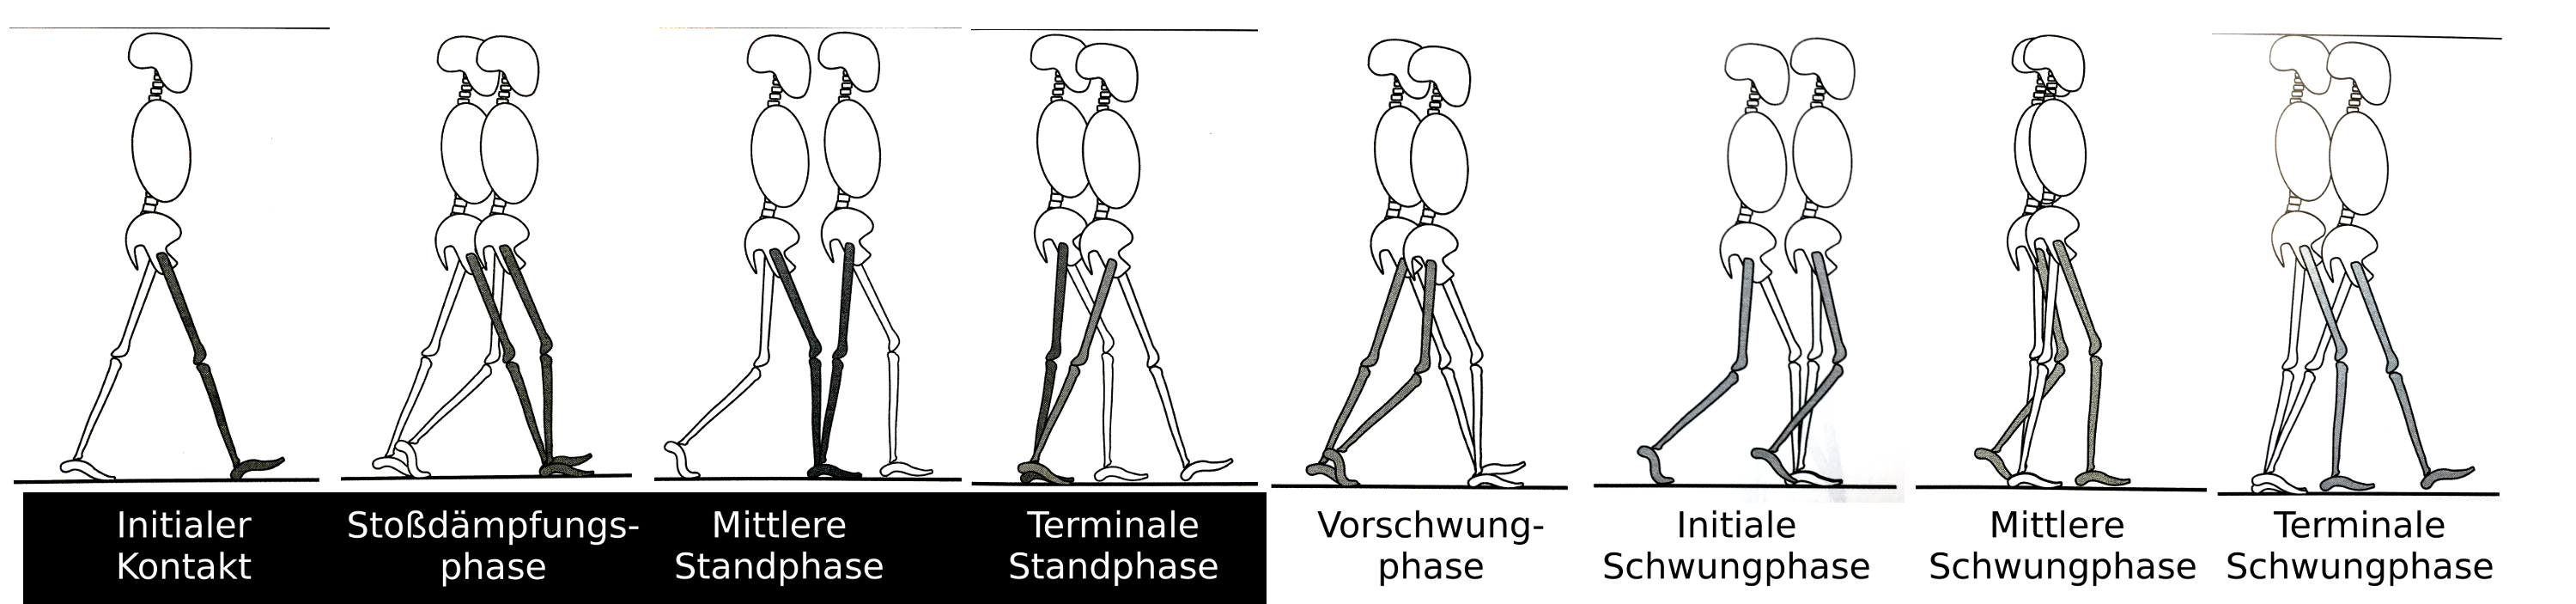
\includegraphics[width=\linewidth]{bilder/Einleitung/Skizze_Gangphasen_small}
	\caption[Gangphasen]{Acht Gangphasen eines Doppelschrittes. Schwarz unterlegt sind die Sub-Phasen der Standphase und grau eingefärbt ist das betrachtete Bein. Veränderte Abbildung nach \autocite{perry2010gait}}
	\label{fig:Skizze_Phasen}
\end{figure}\\
Um den Gangzyklus zu analysieren werden in dieser Arbeit kinematische Analysen von Videomaterial und kinetische Untersuchungen anhand von Bodenreaktionskräften (BRK) durchgeführt. Neben der Identifizierung der oben beschriebenen Gangphasen lassen sich aus den Videos die Dauer der Stand- und Schwungphase ermitteln und mit einem mathematischen Pendel vergleichen. Die Bewegung in der Standphase ähnelt dabei einem inversen Pendel, in der Schwungphase kann das Bein als Gravitationspendel betrachtet werden \parencite{mochon1980ballistic}. Aufgrund der eingangs genannten Besonderheit des fast vollständig gestreckten Beins bleibt der Abstand zwischen Hüftgelenk und Fuß bzw. Massenschwerpunkt in Stand- bzw. Schwungphase dabei annähernd konstant \parencite{witte1992mechanische}. Geht man mit der Geschwindigkeit, bei der die Periodendauer der Stand- oder Schwungphase dem entsprechenden Pendelmodell entspricht, ist für die Fortbewegung ein Minimum an Energie notwendig \parencite{kuo2007six}.\\
Es wird die Hypothese aufgestellt, dass auf der Laufstrecke zusätzlich Energie benötigt wird, um eine Ortsänderung zu erreichen. Es wird vermutet, dass diese Energie aus der Neigung der Körperachse gewonnen wird, wodurch potentielle Energie in kinetische Energie umgewandelt wird. Die kinematischen Untersuchungen auf dem Laufband werden auf der Laufstrecke wiederholt, um die Hypothese zu untersuchen. Dazu werden Hand-Trajektorie, Neigung der Körperachse und Knie-Flexions-Winkel verglichen, um neben dem Hauptkriterium des Körperachsenwinkels noch weitere Parameter einbeziehen zu können.\\
Durch das Messen der Bodenreaktionskräfte (BRK) auf der Laufstrecke können die Lastaufnahme in vertikale und Abbremsen sowie Beschleunigen in horizontale Richtung untersucht werden. Ab einem Verhältnis von Dauer der Standphase zur Dauer des Doppelschrittes von 0.5 ist der Übergang von Gehen zu Laufen definiert. Dieses Verhältnis wird als Duty-Faktor bezeichnet und dient als Maß für die maximale Geh-Geschwindigkeit. Kombiniert man die Daten der Trajektorien von Knöchel, Knie und Hüfte mit den Bodenreaktionskräften so lassen sich mittels inverser Kinetik Kräfte und Momente in den Gelenken ermitteln, ohne Messungen an den jeweiligen Gelenken durchführen zu müssen \parencite{winter2009biomechanics}.\\
Ziel dieser Arbeit ist die korrekte methodische Erfassung der kinematischen und kinetischen Daten und deren Analyse. Dabei wird die inverse Pendeltheorie überprüft und das Laufen auf einem Laufband mit dem Laufen auf einem Laufsteg verglichen. Durch inverse Kinetik werden die Kräfte und Moment im Standbein eines gesunden Mannes analysiert und mit der Literatur verglichen.\\
Aufbauend auf den Ergebnissen werden weiterführende Untersuchungen vorgestellt. Mit den gewonnen Aussagen und den weiterführenden Untersuchungen wird ein Ausblick auf die Übertragbarkeit in die technische Anwendung für Laufroboter und Exoskelette durchgeführt.